\section{Introduction}\label{sect:intro}
The Exascale Computing Project (ECP) Software Technology (ST) focus area represents the key bridge between exascale systems and the scientists who are developing applications that will run on those platforms. The ECP offers a unique opportunity to build a coherent set of software, often referred to as the \textit{software stack}, that will allow application developers to maximize their ability to write highly parallel applications, targeting multiple exascale architectures with runtime environments that will provide high performance and resilience. However, applications are only useful if they can provide scientific insight, and the unprecedented data produced by these applications require a complete analysis workflow that includes new technology to scalably collect, reduce, organize, curate, and analyze the data into actionable decisions. This requires scientific computing to be approached in a holistic manner, encompassing the entire user workflow from problem conception to setting up the problem with validated inputs, performing high-fidelity simulations, to the application of uncertainty quantification to the final analysis. The software stack plan defined here aims to address all of these needs by extending current technologies to exascale, where possible, by performing the research required to create new approaches that address unique problems for which current approaches will not suffice and by deploying high-quality and robust software products on the platforms developed in the exascale systems project.
The ECP ST portfolio has established a set of interdependent projects that will allow a comprehensive software stack to be researched, developed, and delivered, as summarized in Table~\ref{table:wbs}.

\begin{table}
	\begin{tabular}{|>{\columncolor[gray]{0.8}}p{0.10\linewidth}|>{\columncolor[rgb]{0.88,1,1}}p{0.15\linewidth}|p{0.6\linewidth}|}\hline
	    \vfill WBS 2.3.1\vfill & \vfill \centering{Programming Models and Runtimes} \vfill & \vfill Cross-platform, production-ready programming infrastructure to support the development and scaling of mission-critical software at the node and full-system levels.\vfill \\\hline
		\vfill WBS 2.3.2 \vfill & \vfill \centering{Development Tools} \vfill & \vfill A suite of tools and supporting unified infrastructure aimed at improving developer productivity across the software stack. This scope includes debuggers, profilers, and the supporting compiler infrastructure with a particular emphasis on LLVM~\cite{LLVM:2018} as a delivery and deployment vehicle. \vfill \\\hline
		\vfill WBS 2.3.3 \vfill & \vfill \centering{Mathematical Libraries} \vfill & \vfill Mathematical libraries and frameworks that (1) interoperate with the ECP software stack, (2) are incorporated into ECP applications, and (3) provide scalable, resilient, and numerical algorithms that facilitate efficient simulations on exascale computers.\vfill \\\hline
		\vfill WBS 2.3.4 \vfill & \vfill \centering{Data and Visualization} \vfill & \vfill Production infrastructure necessary to manage, share, and facilitate the analysis and visualization of data in support of mission-critical codes. Data analytics and visualization software that support scientific discovery and understanding, despite changes in hardware architecture and the size, scale, and complexity of simulation and performance data produced by exascale platforms. \vfill \\\hline
		\vfill WBS 2.3.5 \vfill & \vfill \centering{Software Ecosystem and Delivery} \vfill & \vfill Development and coordination of software development kits (SDKs) and the Extreme-scale Scientific Software Stack (E4S) across all ECP ST projects.  Development of capabilities in Spack~\cite{gamblin+:sc15} in collaboration with NNSA's primary sponsorship.  Development of SuperContainers~\cite{Supercontainers} and coordination of container-based workflows across DOE computing facilities.\vfill \\\hline
		\vfill WBS 2.3.6 \vfill & \vfill \centering{NNSA ST} \vfill & \vfill Development and enhancement of open-source software capabilities that are primarily developed at Lawrence Livermore, Los Alamos, and Sandia National Laboratories.  Funds for engaging open science application and software teams in the use and enhancement of these products.\vfill \\\hline
	\end{tabular}
	\caption{\label{table:wbs} ECP ST Work Breakdown Structure (WBS), technical area, and description of scope.}
\end{table}

The ECP ST is developing a software stack to meet the needs of a broad set of exascale applications. The current software portfolio covers many projects that span the areas of programming models and runtimes, development tools, mathematical libraries and frameworks, data management, analysis and visualization, and software delivery. The ECP software stack was developed from the bottom up based on application requirements and the existing software stack at US Department of Energy (DOE) high-performance computing~(HPC) facilities. The portfolio comprises projects selected in two different ways.
\begin{enumerate}
\item Thirty projects funded by the DOE Office of Science (SC) as part of the Advanced Scientific Computing Research (ASCR) effort.  This scope of work was selected in October 2016 via a request for information (RFI) and request for proposal (RFP) process that considered prioritized requirements. The initial collection of loosely coupled projects has been reorganized twice and is now in a form that should serve the team well as it moves to the more formal execution phases of the project.
\item Three DOE National Nuclear Security Administration (NNSA) Advanced Simulation and Computing (ASC)-funded projects are part of the Advanced Technology Development and Mitigation (ATDM) program, which was started in FY14 and is now in its sixth year. These projects are focused on longer term research to address the shift in computing technology to extreme, heterogeneous architectures and to advance the capabilities of NNSA ASC simulation codes. 
\end{enumerate}
Since the initial selection process, the ECP ST has reorganized its efforts, as described in Section~\ref{subsect:ProjectRestructuring}.

\begin{figure}
	\centering
	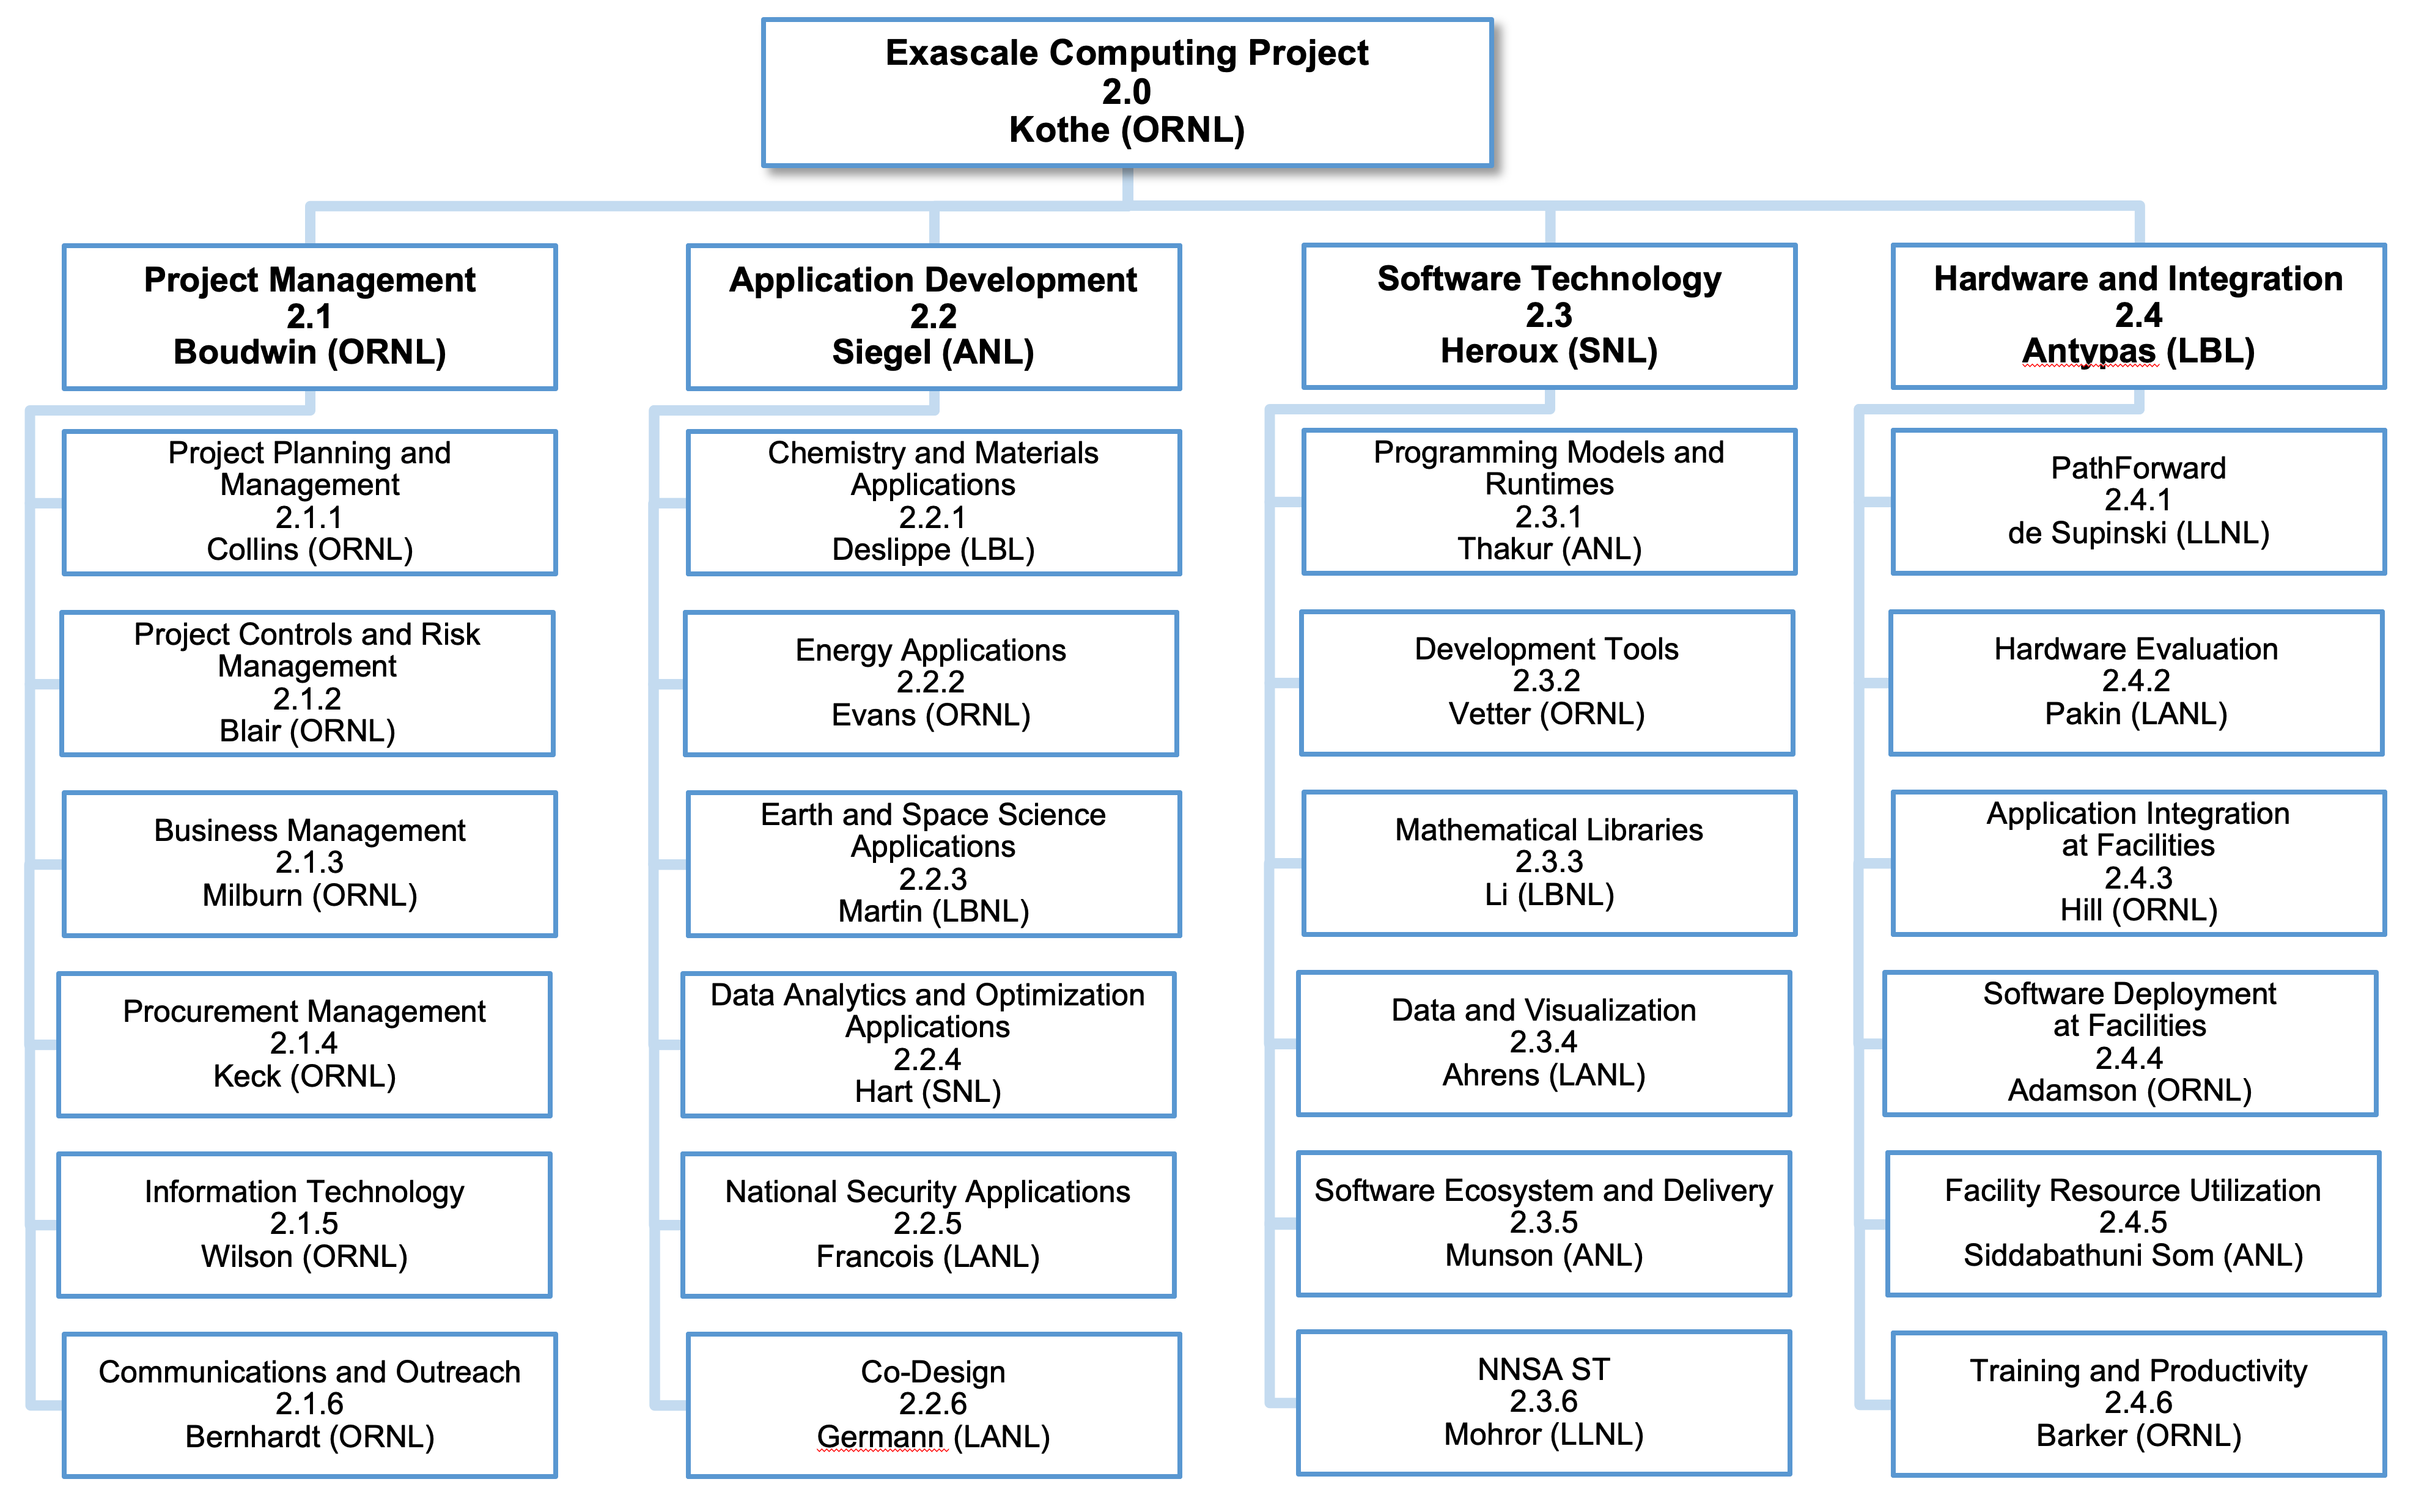
\includegraphics[width=0.9\linewidth]{ECP22}
	\caption{The ECP WBS through Level 3 (L3) as of December 5, 2019. Under ST, WBS 2.3.6 consolidates ATDM contributions to the ECP into a new L3 area.}
	\protect\todo[inline]{Please replace image with higher resolution image that is not a screenshot so that the image is not blurry and no longer has the red spellcheck underline. Also, please add a callout to Figure 1 somewhere in the text.}
	\label{fig:ecp2}
\end{figure}

\subsection{Background}
Historically, the software used on supercomputers has come from three sources: computer system vendors, DOE national laboratories, and academia. Traditionally, vendors have supplied system software, such as operating systems, compilers, runtime, and system-management software. The basic system software is typically augmented by software developed by the DOE HPC facilities to fill gaps or improve system management. System software often breaks or does not perform well when there is a jump in the scale of the system.
 
Mathematical libraries and tools for supercomputers have traditionally been developed at universities and DOE national laboratories and ported to the new computer architectures when they are deployed. Vendors also play a role in this space by optimizing the implementations of commonly used libraries and tools for their architectures while retaining the interfaces defined by the broader community.  This approach enables compile and link time replacement to improve performance on a specific platform by using the vendor versions.  Mathematical libraries and tools have been remarkably robust and have supplied some of the most impactful improvements in application performance and productivity. The challenges have been the constant adapting and tuning to rapidly changing architectures.
 
Programming paradigms and the associated programming environments---which include compilers, debuggers, message passing, and associated runtimes---have traditionally been developed by vendors, DOE laboratories, and universities. The same can be said for file system and storage software. Vendors are ultimately responsible for providing a programming environment and file system with the supercomputer, but vendors are often disinterested in software developed by others or investing in new ideas that have few or no users yet. Also, file system software plays a key role in overall system resilience, and the difficulty of making the file system software resilient has grown nonlinearly with the scale and complexity of the supercomputers.
 
In addition to the lessons learned from traditional approaches, exascale computers pose unique software challenges, including the following.
\begin{itemize}
\item \textbf{Extreme parallelism:} Experience has shown that software breaks at each shift in scale. Exascale systems are predicted to have a billion-way concurrency almost exclusively from discrete accelerator devices, similar to today's GPUs. An alternate approach that uses many cores with vector units is also competitive but still requires the same approximate amount of parallelism.  Because clock speeds have essentially stalled, the 1,000-fold increase in potential performance going from petascale to exascale is entirely from concurrency improvements.
\item \textbf{Data movement in a deep memory hierarchy: }Data movement has been identified as a key impediment to performance and power consumption. Exascale system designs are increasing the types and layers of memory, which further challenges the software to increase data locality and reuse while reducing data movement.
\item \textbf{Discrete memory and execution spaces:} The node architectures of exascale systems include host CPUs and discrete device accelerators.  Programming for these systems requires the coordinated transfer of data and work between the host and device. Although some of this transfer can be managed implicitly, for the most performance-sensitive phases, the programmer typically manages host-device coordination explicitly.  Much of the software transformation effort will focus on this issue.
\end{itemize}
 
In addition to the software challenges imposed by the scale of exascale computers, the following additional requirements push the ECP away from historical approaches of obtaining the needed software for DOE supercomputers.
\begin{itemize}
\item \textbf{2021 acceleration:} One of the ECP's goals is to accelerate the development of the US exascale systems and enable the first deployment by 2021. This means that the software must be ready soon. A concerted plan that accelerates the development of the highest priority and most impactful software is needed.
\item \textbf{Productivity:} Traditional supercomputer software requires considerable expertise to use. One of the ECP's goals is to make exascale computing accessible to a wider science community than was possible with previous supercomputers. This requires developing software that improves productivity and ease of use.
\item \textbf{Diversity:} There is a strong push to make software run across diverse exascale systems. Accelerator devices from NVIDIA have been available for many years, and specific host-device programming and execution applications have been successfully ported to these platforms.  Exascale platforms will continue to have this kind of execution model but with different programming and runtime software stacks.  Writing high-performance, portable code for these platforms will be challenging.
\item \textbf{Analytics and machine learning:} Future DOE supercomputers must solve emerging data science and machine learning problems in addition to the traditional modeling and simulation applications. This will require the development of scalable, parallel analytics and machine learning software for scientific applications, much of which does not exist today.
\end{itemize}
 
\noindent The next section describes the approach the ECP ST used to address the exascale challenges.

\subsection{ECP ST Project WBS changes}\label{subsect:ProjectRestructuring}

The initial organization of the ECP ST was based on discussions that occurred over several years of exascale planning within DOE, especially DOE ASCR.  Figure~\ref{fig:ecpstv1} \todo{Should this be Figure 1? The first 3 figures in this document are not called out. Recommend calling them out prior to this or moving them behind fig:ecpstv1.} shows the conceptual diagram of this first phase.  The 66 ECP ST projects were mapped into eight technical areas, in some cases arbitrating where a project should go based on its primary type of work, even if other work were present in the project.  In November 2017, the ECP ST was reorganized into five technical areas, primarily through merging a few smaller areas, and the number of projects was reduced to 56, then to 55 because of further merging in \ecosystem.  Figure~\ref{fig:ecpstv2} shows the diagram of the second phase of the ECP ST.  Section~\ref{sect:PETA} describes the organization, planning, execution, tracking, and assessment processes that will put the ECP ST in a good position for success in the critical decision (CD) 2 phase of the project.

\begin{figure}
	\centering
	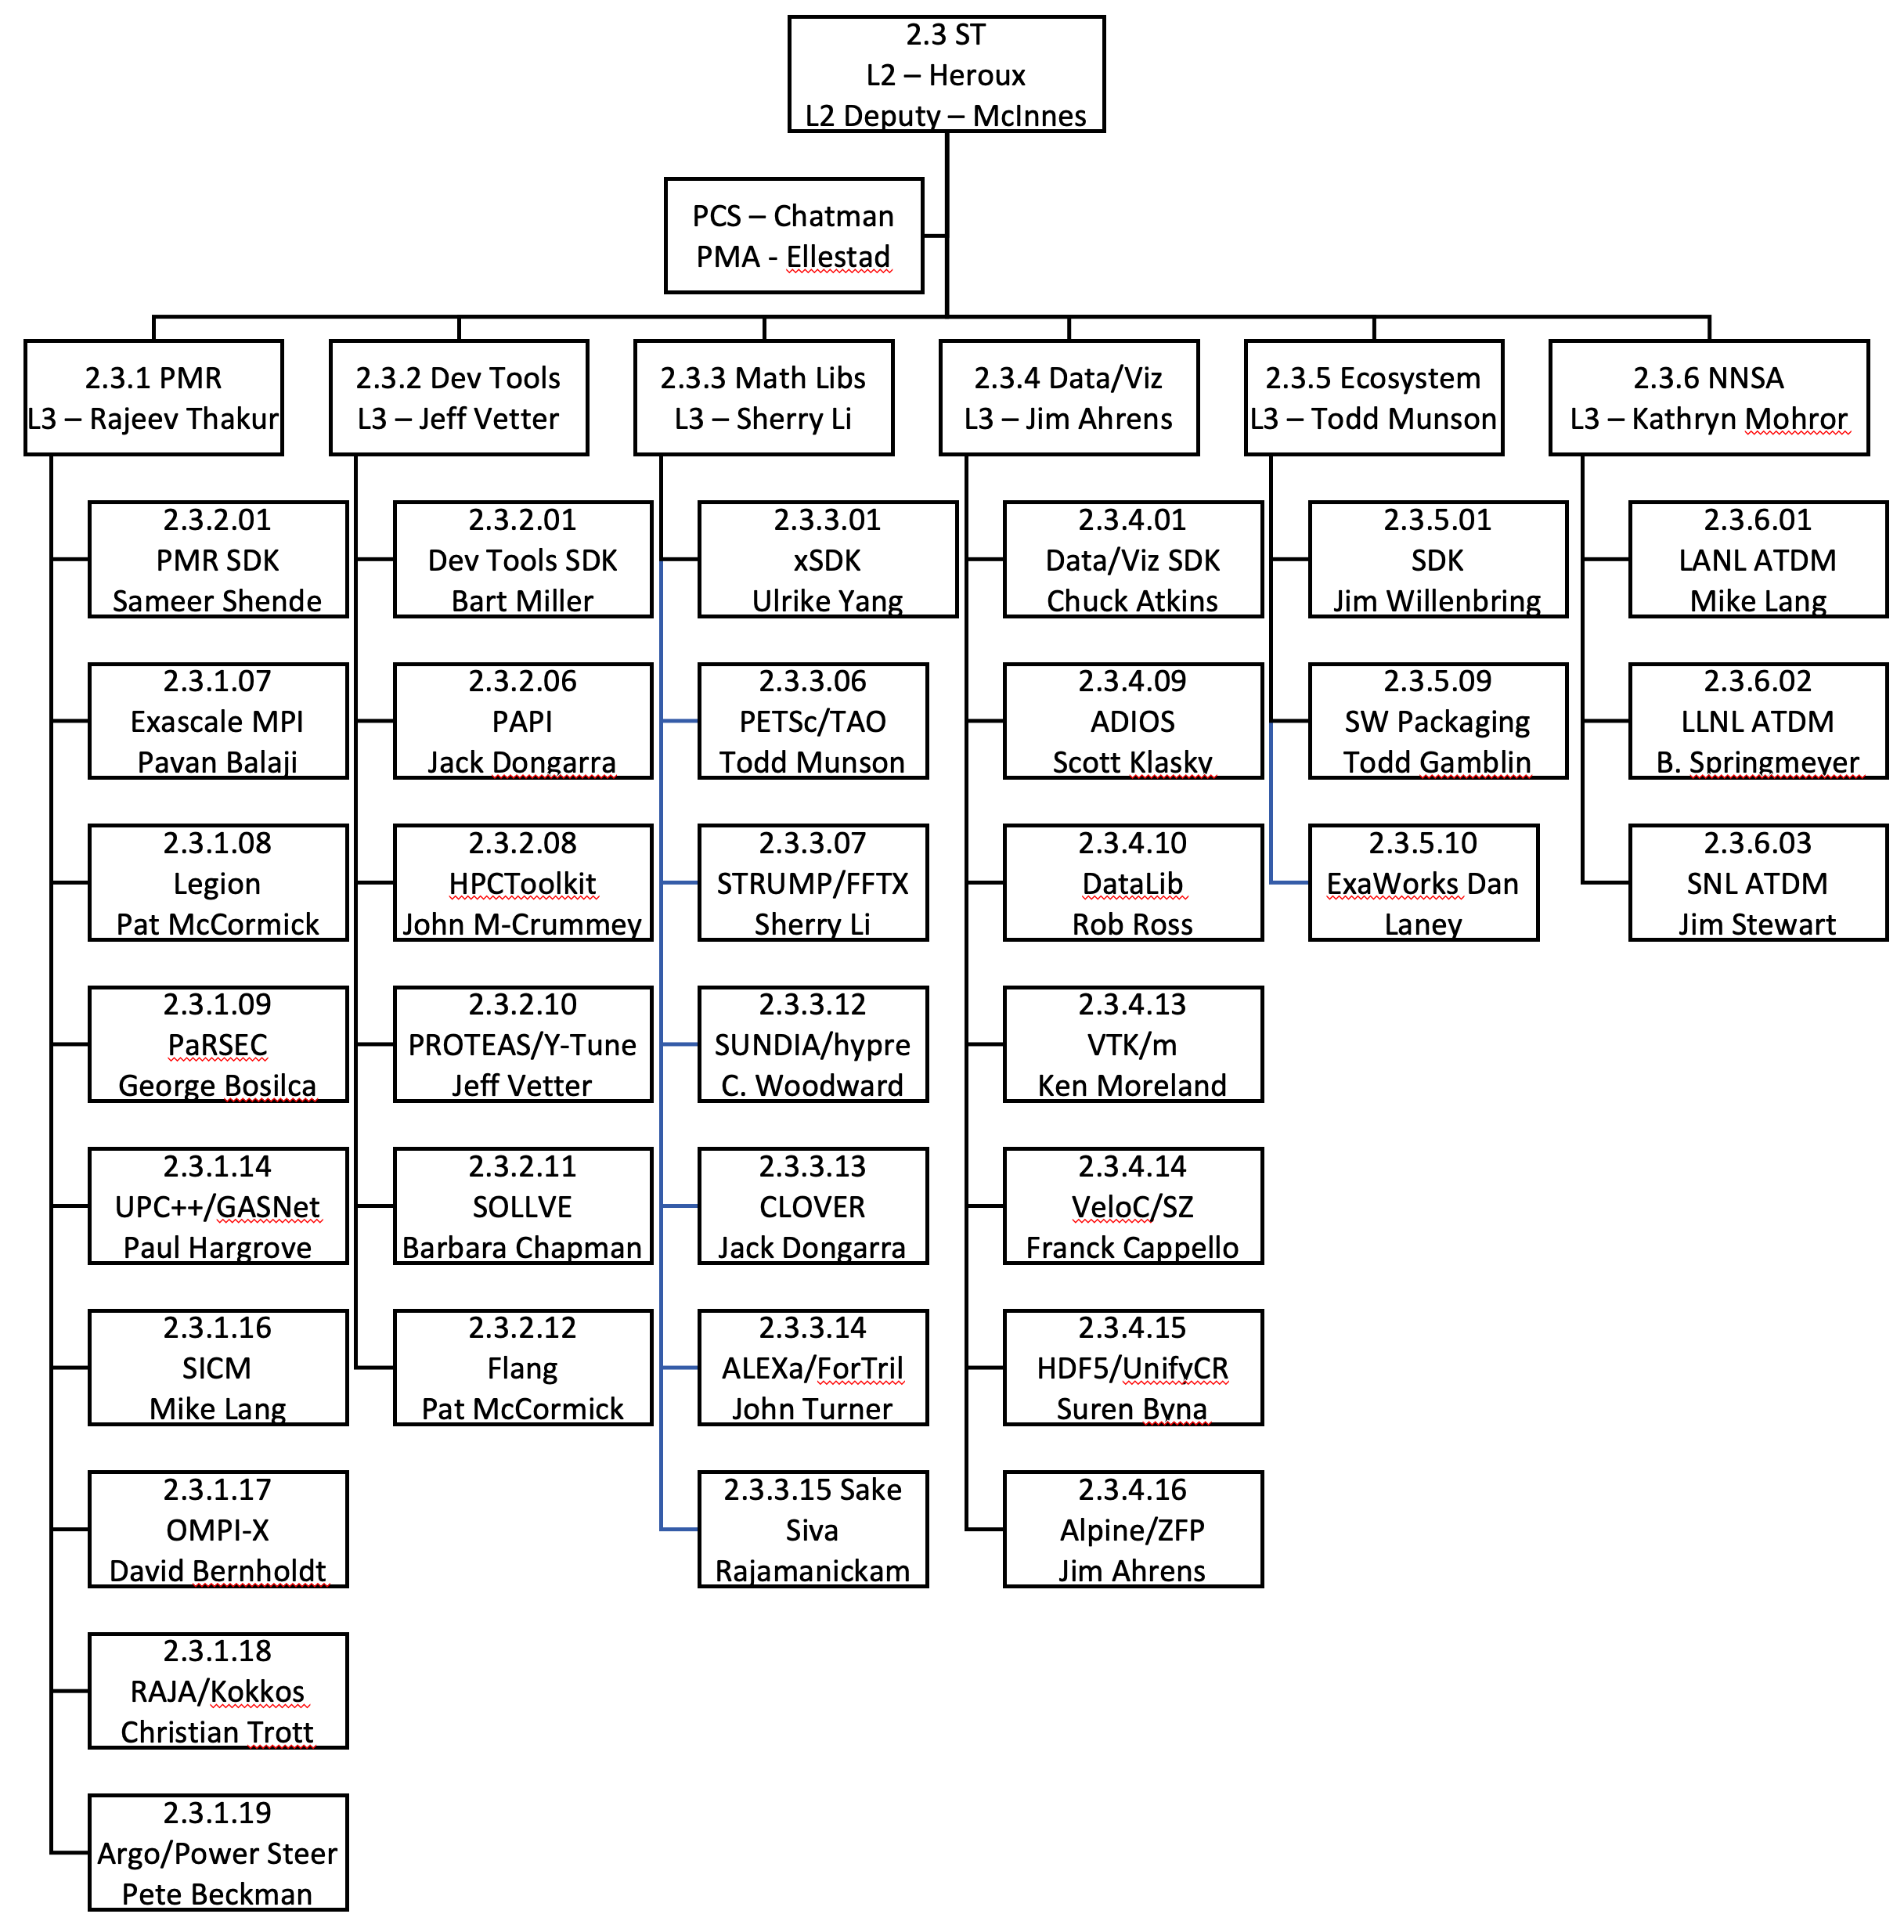
\includegraphics[width=0.9\linewidth]{STFY20WBS}
	\caption{\label{fig:wbs-FY20} The FY20 ECP ST WBS as of November 18, 2020, includes two new Level 4 (L4) subprojects: 2.3.5.10 ExaWorks, a workflow components project, and 2.3.3.15 Sake, a new solver effort that provides funding for Trilinos porting to Frontier and Aurora platforms.}
    \protect\todo[inline]{Please replace image with higher resolution image that is not a screenshot so that the image is not blurry and no longer has the red spellcheck underline.}
\end{figure}

\begin{figure}
\begin{mdframed}
\todo[inline]{Would this be better suited as a list with a header in the narrative?}
\begin{itemize}
\item Phase 1: 66 total L4 subprojects
\begin{itemize}
\item 35 projects funded by DOE SC that were selected in late 2016 via an RFI and RFP process, considering prioritized requirements of applications and DOE facilities. 
These projects started work between January--March 2017, depending on when the contracts were awarded.
\item 31 ongoing DOE NNSA-funded projects that are part of the ATDM program. The ATDM program started in FY14.  These projects are focused on longer term research to address the shift in computing technology to extreme heterogeneous architectures and to advance the capabilities of NNSA simulation codes.
\end{itemize}
\item Phase 2: 55 total L4 subprojects
\begin{itemize}
\item 41 ASCR-funded projects.  Added  two \ecosystem\ projects and four SDK projects.
\item 15 ATDM projects: Combined the previous 31 ATDM projects into one project per technical area per lab.  ATDM projects are generally more vertically integrated and would not perfectly map to any proposed ECP ST technical structure.  Minimizing the number of ATDM projects within the ECP WBS reduces complexity of ATDM to ECP coordination and gives ATDM flexibility in revising its portfolio without disruption to the ECP-ATDM mapping.
\end{itemize}
\item Phase 3a: 33 total L4 subprojects.  Fewer, larger, and more uniform-sized projects.
\begin{itemize}
	\item Starting in FY20, the ECP ST further consolidated L4 projects to foster additional synergies and amortize project overheads as the ECP heads into the CD-2 phase~\cite{413.3B}, in which more rigorous planning and execution are needed.
	\item Five L3s to six: New NNSA ST L3.
	\item 40 ST SC-funded L4 subprojects to 30.
	\begin{itemize}
	\item \pmr: 13 to nine, \tools: six to six, \mathlibs: seven to six, \dataviz: 10 to seven, \ecosystem: four to three.
	\item Includes two new L4 subprojects in \ecosystem.
	\end{itemize}
	\item 15 ST NNSA-funded projects transferred to new NNSA ST L3. Consolidated from 15 to three L4 subprojects.
	\item No more small subprojects.
	\item Figure~\ref{fig:wbs-FY20} shows the overall structure.\todo[inline]{First callout to Figure 2 is within Figure 3. Please correct.}
\end{itemize}
\item Phase 3b: 35 total L4 subprojects.  Add two new L4 subprojects.
\begin{itemize}
	\item New L4 subproject called ExaWorks.  Focuses on providing an underlying component architecture for workflow management systems and is led by a team of workflow experts who would leverage the new substrate in their own workflow products.
	\item New L4 subproject called Sake.  This project was created in response to a need for Trilinos funding to port to Aurora and Frontier.  Concurrently, Trilinos-related activities in the CLOVER project, specifically Kokkos Kernels, were merged with the new Trilinos funding to create a more holistic project independent of CLOVER.
	\item Figure~\ref{fig:wbs-FY20} shows the overall structure.
\end{itemize}
\end{itemize}
\end{mdframed}

\caption{\label{fig:project-remapping}Project remapping summary from Phase 1 (through November 2017) to Phase 2 (November 2017--September 30, 2019) to Phase 3 (After October 1, 2019).}
\end{figure}


\begin{figure}
	\centering
	\includegraphics[width=0.9\linewidth]{ECPSTV1}
	\caption{The ECP ST before the November 2017 reorganization.  This conceptual layout emerged from several years of exascale planning conducted primarily within DOE ASCR.  Because of significant restructuring of the ECP that removed many of the facility's activities and reduced the project time line from 10 to 7 years, as well as a growing awareness of what risks had diminished, this diagram no longer represented the ECP ST efforts accurately.}
	\label{fig:ecpstv1}
	\todo[inline]{Please add a ref to this figure in the narrative.}
\end{figure}
\begin{figure}
	\centering
	\includegraphics[width=0.9\linewidth]{ECPSTV2}
	\caption{The ECP ST after the November 2017 reorganization.  This diagram more accurately reflects the priorities and efforts of the ECP ST given the new ECP project scope and the demands foreseen.}
	\label{fig:ecpstv2}
	\todo[inline]{Please add a ref to this figure in the narrative.}
\end{figure}
\begin{figure}
	\centering
	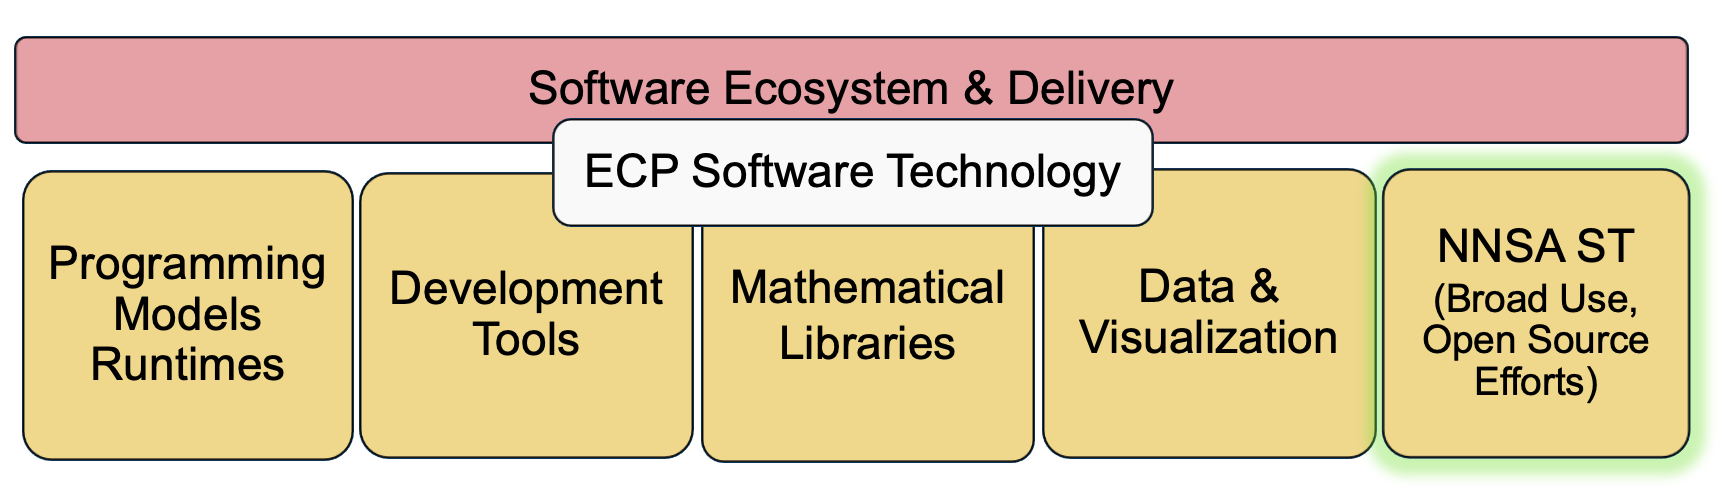
\includegraphics[width=0.9\linewidth]{ECPSTV3}
	\caption{The ECP ST after the October 2019 reorganization.  This diagram reflects the further consolidation of NNSA open-source contributions to enable the more flexible management of NNSA ST contributions.}
	\todo[inline]{Please add a ref to this figure in the narrative.}
\end{figure}
\begin{figure}
	\centering
	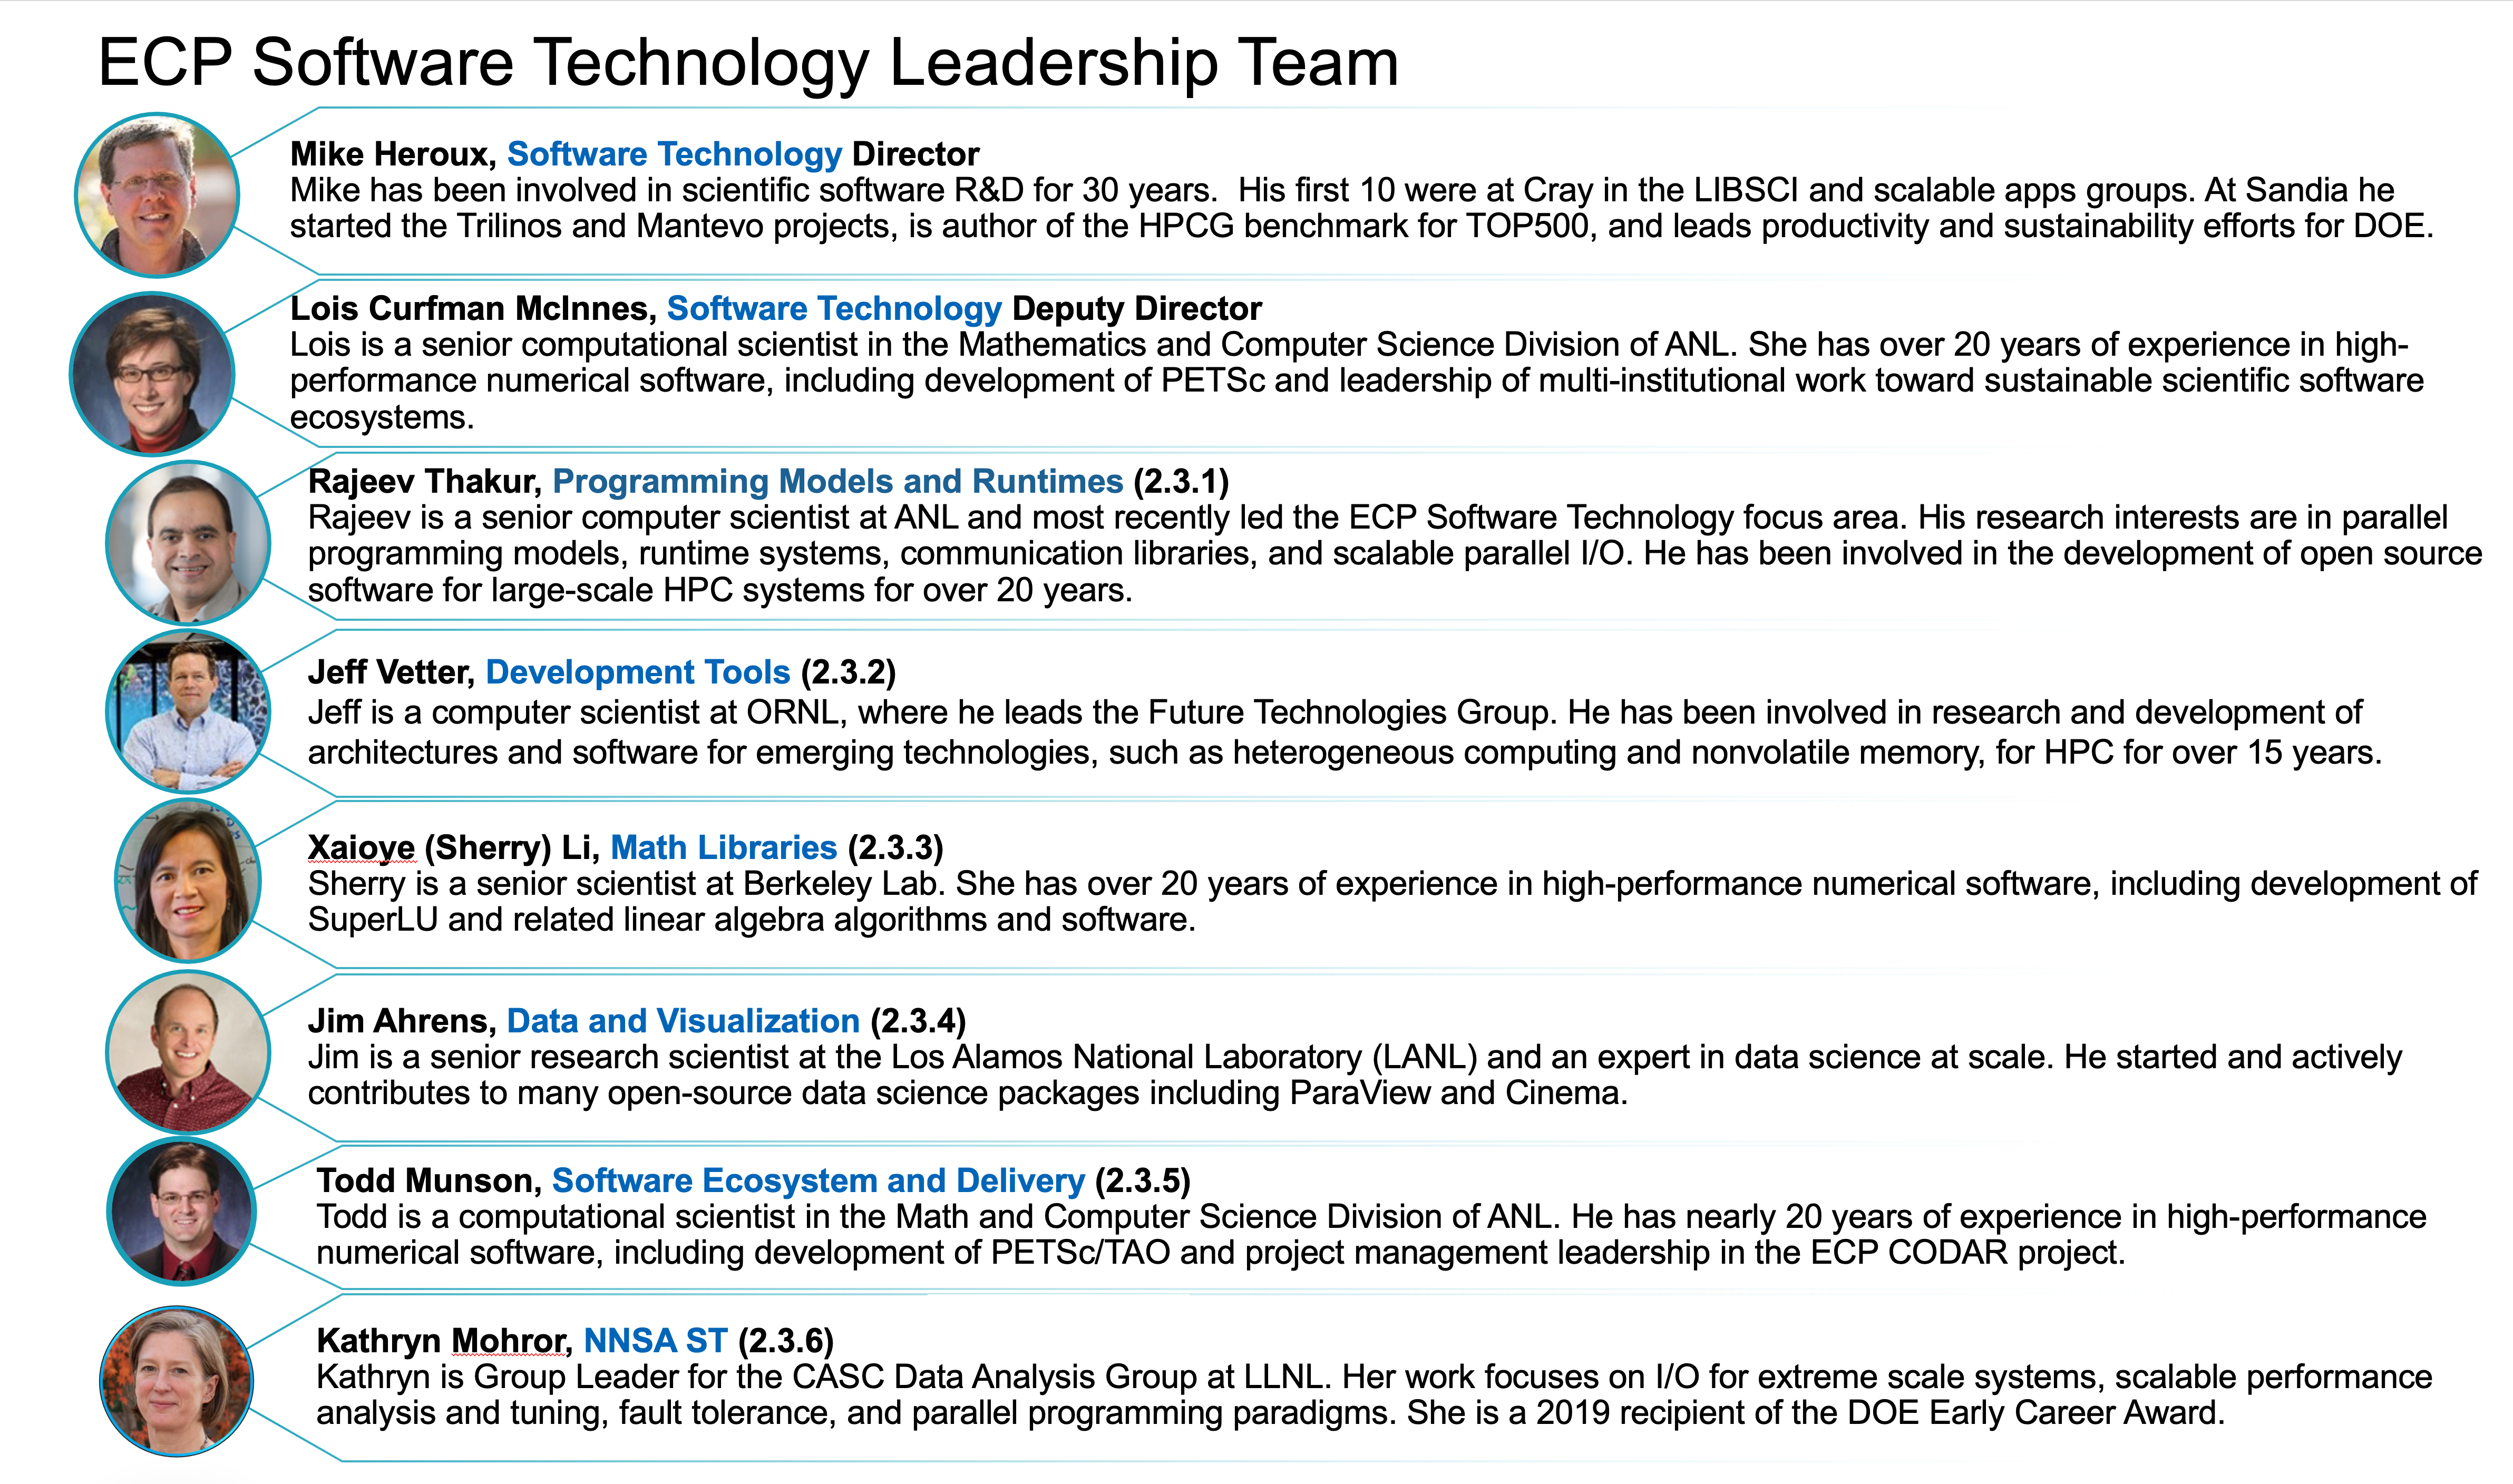
\includegraphics[width=0.9\linewidth]{ECP-ST-Leads}
	\caption{The ECP ST Leadership Team as of November 2020. Jonathan Carter, previous deputy director of the ECP ST, became associate laboratory director of the Computing Sciences Area at Lawrence Berkeley National Laboratory. His departure led to Lois Curfman McInnes, previously the L3 lead of Mathematical Libraries, being named the ECP ST deputy director and Sherry Li being named the new Mathematical Libraries L3 lead.  Rob Neely was also promoted at Lawrence Livermore National Laboratory (LLNL), leading to Kathryn Mohror becoming the L3 lead of NNSA ST.}
	\label{fig:ecpstleads}
	\todo[inline]{Please add a ref to this figure in the narrative.}
\end{figure}

